\documentclass[a4paper,12pt]{report}
\usepackage{styles/fbe_tez}
\usepackage[utf8x]{inputenc} % To use Unicode (e.g. Turkish) characters
\renewcommand{\labelenumi}{(\roman{enumi})}
\usepackage{amsmath, amsthm, amssymb}
 % Some extra symbols
\usepackage[bottom]{footmisc}
\usepackage{cite}
\usepackage{url}
\usepackage{graphicx}
\usepackage{longtable}
\graphicspath{{figures/}} % Graphics will be here

\usepackage{multirow}
\usepackage{subfigure}
\usepackage{algorithm}
\usepackage{algorithmic}

\begin{document}

% Title Page
\title{CMPE 492 \\ Realistic Enough Soft Body Simulation in Virtual Environments for Robotics}
\author{
Asya Su Şen \\ \\
Advisors: \\ 
Atay Özgövde \\
Müge Taşkın \\
Emre Uğur
}
\date{}
\maketitle{}
\pagenumbering{roman}
\tableofcontents

\chapter{INTRODUCTION}
\pagenumbering{arabic}

\section{Broad Impact}
The integration of robotics into complex, unstructured environments relies heavily on the ability of autonomous agents to interact seamlessly with deformable objects. While rigid body dynamics have been extensively studied and optimized for real-time applications, soft body dynamics—encompassing cables, ropes, fabrics, and organic tissues—remain a significant computational challenge. The broad impact of this project lies in narrowing the "Sim2Real" (Simulation to Reality) gap specifically for soft body manipulation tasks. 

Training machine learning models, particularly Deep Reinforcement Learning (DRL) agents, directly on physical hardware is often prohibitively expensive, time-consuming, and prone to causing hardware damage during the exploratory phases of learning. Consequently, the standard paradigm relies on training agents within virtual physics simulators and subsequently transferring the learned policies to real-world robots. However, if a simulation lacks physical fidelity, the AI will inevitably learn to exploit mathematical inaccuracies—such as tunneling through collision meshes or generating infinite forces from joint instabilities. Conversely, utilizing rigorous engineering-grade solvers like the Finite Element Method (FEM) provides ground-truth accuracy but at a computational cost that makes iterative AI training impossibly slow. 

This project directly addresses this bottleneck by developing a framework for "realistic enough" physics simulations within the Unity engine. By carefully balancing computational efficiency with physical plausibility, the resulting environments run fast enough to support massive parallel training loops while retaining the geometric and dynamic constraints necessary for successful Sim2Real transfer. 

Furthermore, this project establishes a flexible, two-way feedback pipeline with the COLORS Lab. Rather than producing a single, static simulation, the framework is designed to be highly agile. As the laboratory's research needs evolve, new environments and soft-body constraints are rapidly prototyped, simulated, and refined. While current implementations feature scenarios such as an RCA cable and socket interaction, the underlying architecture is not restricted to specific hardware. This iterative approach ensures that the simulated environments directly accelerate the lab's ongoing robotics research, empowering researchers to test novel manipulation algorithms on varied, highly optimized soft body scenarios before any real-world deployment occurs.

\section{Ethical Considerations}
As this project directly facilitates the training of robotic agents for physical deployment, several ethical considerations must be addressed regarding safety, environmental impact, and the predictability of autonomous systems.

First and foremost is the issue of AI safety and physical unpredictability. Policies trained in virtual environments are fundamentally constrained by the limitations of the underlying physics engine. If an agent is trained to manipulate a simulated cable that does not accurately model tension limits or shear forces, the physical robot may attempt to apply excessive force in reality. When dealing with electrical cables, delicate components, or in environments shared with humans, such erratic behavior can lead to severe hardware damage, electrical hazards, or physical injury. Ensuring that the "realistic enough" threshold successfully captures critical failure states and prevents the agent from learning dangerous edge-case behaviors is a paramount ethical responsibility. The simulations must accurately penalize unsafe manipulations so that the AI learns respect for the physical limitations of soft bodies.

Secondly, the computational efficiency of the simulation framework carries environmental implications. Training modern machine learning models requires massive computational power, contributing to the growing carbon footprint of artificial intelligence research. By deliberately optimizing the soft body simulations to maximize frame rates and reduce unnecessary processing overhead—without compromising necessary physical constraints—this project supports more sustainable and energy-efficient training pipelines. Creating lightweight simulations ensures that high-quality robotics research can be conducted without demanding excessive data center resources.

Finally, advancing the capabilities of robotic manipulation in unstructured environments accelerates the automation of complex manual tasks. While this effectively removes humans from hazardous or repetitive work environments, it also contributes to ongoing shifts in the labor market. Acknowledging the socioeconomic impact of transferring traditionally human-operated tasks—such as complex cable routing, electronics assembly, or delicate material handling—to autonomous systems is an essential aspect of developing responsible and forward-looking robotics technologies.

\chapter{PROJECT DEFINITION AND PLANNING}
\section{Project Definition}
The primary objective of this project is to develop a highly optimized, physically plausible simulation framework for soft body dynamics—specifically focusing on one-dimensional deformable objects such as cables, wires, and ropes—within the Unity engine. The core engineering challenge lies in balancing two inherently conflicting requirements: computational efficiency and physical realism. Standard engineering solvers, such as the Finite Element Method (FEM), offer high fidelity but cannot achieve the frame rates required for massive, parallel training of machine learning agents. Conversely, standard game engine physics often lack the rigorous constraint solving necessary to prevent collision tunneling, explosive corrective forces, or joint instability during complex robotic manipulation. 

Therefore, this project precisely targets the "realistic enough" operational threshold. The goal is to construct environments that compute fast enough to support Deep Reinforcement Learning (DRL) algorithms, while maintaining the essential structural, geometric, and collision integrity required to prevent Sim2Real transfer failures. 

Rather than building a single static simulation, this project is defined as an adaptive, two-way physics pipeline developed in direct collaboration with the Cognitive Learning and Robotics (COLORS) Lab. The specific soft bodies, physics thresholds, and environmental constraints simulated are dynamically driven by the evolving empirical needs of the lab's researchers. The framework functions as an agile testbed where novel robotic manipulation tasks can be quickly prototyped, safely verified, and optimized before any deployment on physical hardware occurs.

\section{Project Planning}
Given the research-oriented and collaborative nature of this work, a rigid, traditional waterfall planning model is ineffective. Instead, the project employs an iterative, agile planning methodology. The development cycle is tightly coupled with the feedback loop from the COLORS Lab. As researchers define new manipulation tasks or encounter specific physical edge-cases in their AI training pipelines, the simulation parameters, constraint solvers, and environments are actively adjusted to meet those exact specifications. This flexible planning structure ensures that development time is strictly allocated to delivering simulation features that directly accelerate the lab's active research goals.

\subsection{Project Time and Resource Estimation}
The fundamental resources for this project are computational. The primary development environment is the Unity Engine, utilizing custom C\# scripting, the native physics backend (including Articulation Bodies), and various custom constraint solvers. Version control is strictly managed via Git and GitHub to maintain a stable, modular repository of physics experiments, allowing different environments to be branched and tested independently. Hardware resources consist of standard consumer-grade hardware, which acts as a practical benchmark for verifying the simulation's computational efficiency; if the simulation runs optimally here, it scales excellently in cloud-based AI training clusters.

The project timeline is structured around iterative development milestones:
\begin{itemize}
    \item \textbf{Phase 1: Literature Review and Theoretical Grounding (Completed):} Extensive comparative research into 1D soft body simulation techniques—including Position-Based Dynamics (PBD), Continuum Mechanics (FEM), Multi-Body Dynamics, and Procedural Splines—and their respective computational overheads.
    \item \textbf{Phase 2: Baseline Implementation and Prototyping (Completed/Ongoing):} Initial practical testing of external solvers and native implementations of multi-body joint chains. This resulted in the current baseline stable simulation utilizing Articulation Bodies and mixed constraints (e.g., the RCA cable and socket plugging scenario).
    \item \textbf{Phase 3: Iterative COLORS Lab Integration (Ongoing):} The core active phase, consisting of rapid prototyping cycles. Environments are customized based on the immediate specifications of the COLORS Lab, profiled for computational efficiency, and refined based on how well AI agents can interact with the simulated soft bodies.
    \item \textbf{Phase 4: Final Optimization and Documentation (Future):} A final optimization pass to maximize the frame-rate-to-realism ratio, quantitative profiling of the physics overhead, and the completion of the final thesis report.
\end{itemize}
\subsection{Success Criteria}
Because this project serves as a foundational tool for machine learning research rather than a standalone commercial game, its success is measured by its utility, stability, and performance within an AI training pipeline. The project will be considered successful if it meets the following criteria:

\begin{itemize}
    \item \textbf{Physics Stability and Robustness:} The soft body simulations (specifically cables and joint chains) must not exhibit catastrophic numerical instability—commonly referred to as "physics explosions." The bodies must handle high-velocity impacts, sudden tension, and complex environmental wrapping without the constraint solver failing or causing severe geometry clipping/tunneling.
    \item \textbf{Computational Efficiency:} The simulation must consistently maintain a frame rate and physics calculation step fast enough to support iterative Reinforcement Learning. While FEM-level accuracy is sacrificed, the "realistic enough" calculations must not become a bottleneck that prevents massive parallel training.
    \item \textbf{Physical Plausibility (Sim2Real Viability):} The simulated objects must exhibit emergent physical properties vital for manipulation, such as resting friction, torsional resistance, and appropriate bend radii. For example, a simulated cable must resist folding perfectly flat if its physical counterpart has high stiffness.
    \item \textbf{COLORS Lab Integration:} The ultimate metric of success is adoption. The framework must successfully allow COLORS Lab researchers to prototype a robotic manipulation task (such as the RCA cable insertion or general cable routing) and extract meaningful interaction data or train a baseline control policy. 
\end{itemize}

\subsection{Risk Analysis}
Developing custom physics simulations inherently carries significant technical risks, primarily revolving around the trade-off between speed and accuracy.

\begin{itemize}
    \item \textbf{Risk 1: Inherent Multi-Body Instability.} Traditional game engine physics using force-based constraints ($F=ma$) often fail when simulating long chains of small, connected rigid bodies (like a discretized cable). High tension can cause the joints to separate or generate infinite corrective forces. \textit{Mitigation:} Utilizing reduced-coordinate formulations (like Unity's ArticulationBody with Featherstone's algorithm) or migrating entirely to geometric Position-Based Dynamics (PBD/XPBD) to guarantee unconditional mathematical stability.
    \item \textbf{Risk 2: Performance Degradation from Collision Detection.} Soft bodies require continuous, self-aware collision detection across many nodes, which scales poorly ($O(N^2)$). \textit{Mitigation:} Implementing localized collision layers, using thick continuous collision detection (CCD) capsules only where strictly necessary, and offloading constraint solving to Unity's multithreaded Job System and Burst Compiler.
    \item \textbf{Risk 3: Scope Creep via Lab Feedback.} Because the project is highly responsive to the evolving needs of the COLORS Lab, there is a risk of continuous redesigns preventing the finalization of a stable build. \textit{Mitigation:} Enforcing a strictly modular architecture. The core physics solver and soft-body mathematical framework are kept entirely decoupled from the specific 3D meshes and environmental scenarios requested by the lab.
\end{itemize}

\subsection{Team Work (if applicable)}
-
\chapter{RELATED WORK}

\section{General Soft Body Simulation Techniques}
The simulation of deformable objects in virtual environments spans a spectrum of methodologies, balancing high-fidelity engineering models with hyper-optimized visual approximations. A comprehensive review of current techniques reveals 10 primary approaches utilized within the Unity engine, each presenting distinct trade-offs between physical accuracy and computational efficiency. 

Table \ref{table:comparisonMatrix} summarizes these techniques, highlighting their primary strengths, disadvantages, and ideal use cases within robotics.

\begin{table}[thbp]
\vskip\baselineskip 
\caption{Comparison Matrix of Soft Body Simulation Techniques}
\begin{center}
\begin{tabular}{|p{2.5cm}|p{3.5cm}|p{3.5cm}|p{3.5cm}|} \hline
 \textbf{Technique} & \textbf{Primary Strength} & \textbf{Primary Disadvantage} & \textbf{Ideal Robotics Use Case} \\\hline
 \textbf{FEM (Physical)} & Highest physical accuracy and stress/strain data. & Extreme computational load; needs volumetric meshes. & Surgical simulation and precision robotics. \\\hline
 \textbf{PBD (Geometric)} & Exceptional stability; mathematically immune to explosions. & Stiffness is iteration-dependent. & Stable grasping and reliable manipulation. \\\hline
 \textbf{Mass-Spring} & Computational efficiency; easy to script. & Numerical instability; lacks volume conservation. & Fast, simple tactile sensor skin approximation. \\\hline
 \textbf{MPM (Hybrid)} & Handles cutting, tearing, and melting seamlessly. & High memory bandwidth; grid-resolution dependent. & Simulating the cutting of biological tissues. \\\hline
 \textbf{ARAP} & Preserves artistic and visual detail. & No internal pressure or material properties. & Visual feedback for manual teleoperation. \\\hline
 \textbf{Neural (GNN)} & Learns complex, un-programmable friction. & Black box nature; requires massive datasets. & Sim2Real transfer when real data exists but math models lack. \\\hline
 \textbf{ROM} & FEM-level accuracy at real-time speeds. & Cannot handle states outside the training set. & High-speed robot control loops (fixed deformation range). \\\hline
 \textbf{Shape Matching} & Unconditional stability; works with point clouds. & Artificial, rubbery feel; limited accuracy. & Fast prototyping from point-cloud data. \\\hline
 \textbf{Bone Physics} & Extreme performance; animation compatible. & Non-physical; no volume preservation. & Secondary dynamics (VR/Mobile). \\\hline
 \textbf{Unity Cloth} & Optimized native C++ performance. & Strictly limited to 2D surfaces (shells). & Thin fabrics or protective sleeves. \\\hline
\end{tabular}
\label{table:comparisonMatrix}
\end{center}
\end{table}

\subsection{Implementation Frameworks and Selection Logic}
Within the Unity ecosystem, these techniques are typically powered by two core backend frameworks. Compute Shaders (GPU) provide massive scalability, ideal for handling hundreds of thousands of particles in parallel (e.g., dense PBD or Mass-Spring systems). Conversely, the Job System and Burst Compiler (CPU)—the core of Unity's Data-Oriented Technology Stack (DOTS)—provide native-speed, multithreaded performance. This is particularly ideal for PBD or Bone Physics when CPU tasks, such as Artificial Intelligence processing and Robot Operating System (ROS) communication, must run concurrently.

Selecting the appropriate solver is entirely dependent on the required data output. The Finite Element Method (FEM) is strictly required when rigorous internal stress and strain metrics are necessary. For real-time interaction without "explosive" physics, geometric approaches like Position-Based Dynamics (PBD) are favored over standard Mass-Spring systems. When training an AI agent, techniques like Reduced Order Modeling (ROM) or Neural Simulators are preferred, as they provide the high-speed, low-dimensional states crucial for efficient Reinforcement Learning.

\section{1D Soft Body Simulation (Cables and Ropes)}
Simulating one-dimensional soft bodies, such as cables, ropes, and strings, in real-time requires specific architectural considerations to balance interaction fidelity with continuous mechanics. Current industry and academic approaches can be categorized into five primary methods.

\subsection{Procedural Splines and Spring-Dampers}
This method bypasses continuous physics, rendering the cable as a mathematical curve (e.g., a Rational Bezier Curve) evaluated between anchor points. Instead of simulating $N$ nodes, the physics engine evaluates a single midpoint using a damped harmonic oscillator model:
$$F=-kx-cv$$
This central point calculates a target resting position based on gravity, applies stiffness $k$ to calculate acceleration, and uses damping $c$ to dissipate kinetic energy.
\begin{itemize}
    \item \textbf{Industry Application:} Utilized heavily in VR (e.g., \textit{Half-Life: Alyx}), where mathematical curves are paired with thick Continuous Collision Detection (CCD) capsules.
    \item \textbf{Trade-offs:} Offers extremely low CPU overhead (an $O(1)$ physics cost relative to cable length). However, it is fundamentally incapable of true self-collision, complex wrapping, or knotting.
\end{itemize}

\subsection{Multi-Body Dynamics (Articulation Bodies)}
This standard rigid-body approach discretizes the cable into a kinematic chain of rigid segments (capsule colliders) linked via rotational constraints. Modern robotics engines utilize Featherstone's algorithm to solve this kinematic chain in reduced coordinates. This computes the forward dynamics of the entire multi-body system in $O(N)$ time, avoiding the joint separation inherent in traditional impulse-iteration solvers. While it provides exact, native collision detection with rigid end-effectors, it scales poorly with high segment counts and remains susceptible to tunneling at high velocities.

\subsection{Position-Based Dynamics (PBD) and Extended PBD (XPBD)}
PBD abandons standard force-based formulations. The cable is modeled as a 1D array of point masses connected by constraints (Distance, Bending, and Pin constraints). The solver integrates velocities to find predicted positions, then iteratively projects these positions to satisfy geometric rules. XPBD improves upon basic PBD by introducing compliance (inverse stiffness) proportional to $\Delta t^2$, decoupling the cable's simulated stiffness from the engine's frame rate and iteration count. This method is unconditionally stable and highly capable of complex wrapping and knotting, though it incurs a high CPU cost across multiple iterations.

\subsection{Continuum Mechanics (FEM)}
FEM models the cable as a continuous 3D volumetric mesh (typically tetrahedrons) rather than a 1D line. It calculates internal stress and strain by solving the dynamic system:
$$M\ddot{\mathbf{u}}+D\dot{\mathbf{u}}+\mathbf{f}_{int}(\mathbf{u})=\mathbf{f}_{ext}$$
Here, internal forces ($\mathbf{f}_{int}$) derive directly from real-world parameters like Young's Modulus and Poisson's Ratio. While providing the absolute highest fidelity for Sim2Real transfer (capturing shear, torsion, and volume preservation), the non-linear calculations are mathematically complex and often require external frameworks or Reduced Order models for real-time execution.

\subsection{Custom Soft-Body Solvers and Animation Blending}
In scenarios where standard methods fail to meet specific interactive criteria, bespoke solvers are paired with animation data. For instance, in \textit{The Last of Us Part II}, a custom algorithm was engineered to calculate exactly how a taut rope bends and anchors around complex collision geometry (like brick corners). Furthermore, when the simulated rope reaches maximum tension, the physics engine directly triggers Inverse Kinematics (IK) in the character's animation controller to physically lock the arm, transferring simulated tension into visual, kinematic weight.
\chapter{METHODOLOGY}
\section{System Architecture and Framework}
The core objective of this project is to construct a highly optimized, physically plausible environment for Sim2Real robotic training. To achieve this, the simulation architecture is built upon the Unity engine, utilizing custom C\# parametric generators rather than relying strictly on default physics components. 

The architecture is designed to be highly modular, separating the mathematical calculation of the soft body's shape from its visual rendering and its interactive endpoints. This decoupling allows researchers at the COLORS Lab to rapidly generate various cable scenarios by modifying top-level parameters—such as length, slack, and control point weighting—without altering the underlying solver. The system framework consists of three primary layers: the mathematical solver (evaluating spatial coordinates), the visual layer (rendering the continuous mesh), and the interaction layer (handling specific manipulation tasks, such as end-effector socket triggers).

\section{Mathematical Modeling of Linear Deformable Objects}
Through an iterative evaluation of multiple physics solvers—including Position-Based Dynamics (PBD) and reduced-coordinate Multi-Body Dynamics—it was determined that traditional continuous constraint solvers introduce severe computational bottlenecks that hinder massive parallel AI training. Therefore, the selected optimal methodology employs a Procedural Kinematics approach, specifically utilizing Rational Bezier Curves.

Instead of discretizing the cable into a heavy kinematic chain of rigid bodies subject to standard Newtonian forces ($F=ma$), the cable is modeled as a mathematical curve driven by isolated physical control points. For a standard cubic Bezier curve, the position of any point $B(t)$ along the cable is evaluated using the explicit formulation:
$$B(t) = (1-t)^3 P_0 + 3(1-t)^2 t P_1 + 3(1-t) t^2 P_2 + t^3 P_3 \quad \text{for } 0 \le t \le 1$$
Where $P_0$ through $P_3$ represent the localized spatial coordinates of the anchor points, tangent handles, and the cable's dynamic midpoint. 

To simulate gravity and tension without calculating $N$-node interactions, physics computations are strictly limited to the control points. The central dynamic point can be approximated using a damped harmonic oscillator model, ensuring that the cable visually reacts to momentum and gravity while maintaining an $O(1)$ calculation cost relative to the total length of the simulated object.

\section{Simulation Setup and End-Effector Interaction}
Translating this mathematical model into a functional simulation involves specific programmatic structures to handle generation, visualization, and manipulation.

\begin{itemize}
    \item \textbf{Parametric Generation (\texttt{BezierCableGenerator.cs}):} The physical length and baseline slack of the cable are procedurally generated upon initialization. Anchor points are established at the environment's origin and the end-effector (such as an RCA plug), with dynamic tangent vectors continuously calculating the required curvature based on the spatial distance between the two ends.
    \item \textbf{Visual Smoothing (\texttt{SmoothCableVisuals.cs}):} Because the mathematical model only calculates the high-level spline trajectory, the visual fidelity is interpolated locally. A LineRenderer dynamically interpolates $N$ graphical segments along the defined $B(t)$ curve, creating a smooth, continuous surface without adding active colliders to every segment.
    \item \textbf{Task-Specific Triggers (\texttt{SocketTrigger.cs}):} A major requirement for robotic manipulation is precise end-effector interaction. Since the procedural spline lacks continuous self-collision, interaction is localized to the rigid end-effectors. For specific tasks like connecting an RCA cable, volumetric trigger colliders are utilized at the socket destination. The simulation mathematically evaluates the orientation and proximity of the plug's rigid body to the socket's transform, executing customized connection logic (snapping or locking) only when positional thresholds are met.
\end{itemize}

\section{Evaluation and Selection Criteria}
The primary metric for validating this methodology is the "realistic enough" threshold: the ratio of computational efficiency to interactive stability. 

While rigorous engineering methods like the Finite Element Method (FEM) offer perfect stress and strain metrics, they operate at frame rates far too slow for Reinforcement Learning pipelines. Conversely, Multi-Body Dynamics often suffer from "explosions" (infinite corrective forces) when high-velocity movements stretch the simulated joints beyond their limits. 

The procedural Bezier spline methodology was ultimately selected as the optimal solution because it fundamentally guarantees absolute mathematical stability. By removing inter-particle collision layers and resolving the cable's shape kinematically, the environment maintains exceptionally high frame rates, completely eliminating the risk of joint-chain explosions during violent or erratic manipulation attempts by an untrained AI agent. This ensures that the training loop remains uninterrupted while still providing the necessary visual and endpoint interaction data required for successful policy transfer to physical hardware.

\chapter{REQUIREMENTS SPECIFICATION}
The requirements specification for the Realistic Enough Soft Body Simulation framework outlines the functional interactions between the primary actors and the system. Unlike traditional software applications, the "users" of this system include both human researchers and autonomous machine learning agents.

\section{Actor Identification}
\begin{itemize}
    \item \textbf{COLORS Lab Researcher:} The human operator who defines the physical parameters of the soft body, establishes the environmental constraints, and evaluates the success of the simulation.
    \item \textbf{DRL Agent (AI):} The Deep Reinforcement Learning algorithm that acts as an autonomous user within the Unity environment, iteratively interacting with the soft body to learn manipulation policies.
\end{itemize}

\section{Use Case Descriptions}
The agile, two-way feedback pipeline is defined by an iterative set of core use cases, effectively bridging the Sim2Real gap:

\begin{itemize}
    \item \textbf{UC1: Configure Unity Environment:} The Researcher inputs specific parameters (e.g., cable length, stiffness, procedural spline anchors) into the Unity framework via the parametric generators.
    \item \textbf{UC2: Execute Virtual Training:} The DRL Agent interacts with the generated soft body environment, executing thousands of iterations to learn a baseline manipulation policy safely.
    \item \textbf{UC3: Evaluate and Refine Physics (Retinker):} The Researcher evaluates the agent's virtual performance. If the physics are deemed unrealistic (e.g., the agent exploits mathematical tunneling) or if initial physical tests fail, the Researcher returns to UC1 to adjust the solver constraints and generate a new environment.
    \item \textbf{UC4: Deploy to Physical Hardware:} Once the policy is stable and the physics are deemed "realistic enough" without performance bottlenecks, the Researcher deploys the trained DRL Agent onto the physical robotic hardware in the real world.
\end{itemize}

\section{Use Case Diagram}
The interactions described above are visualized in the iterative Sim2Real Use Case Diagram (Figure \ref{fig:usecase}). The diagram illustrates the cyclical feedback loop where the Unity simulation acts as the central bridge between initial configuration, continuous retraining, and final real-world deployment.

\begin{figure}[h!]
\centering

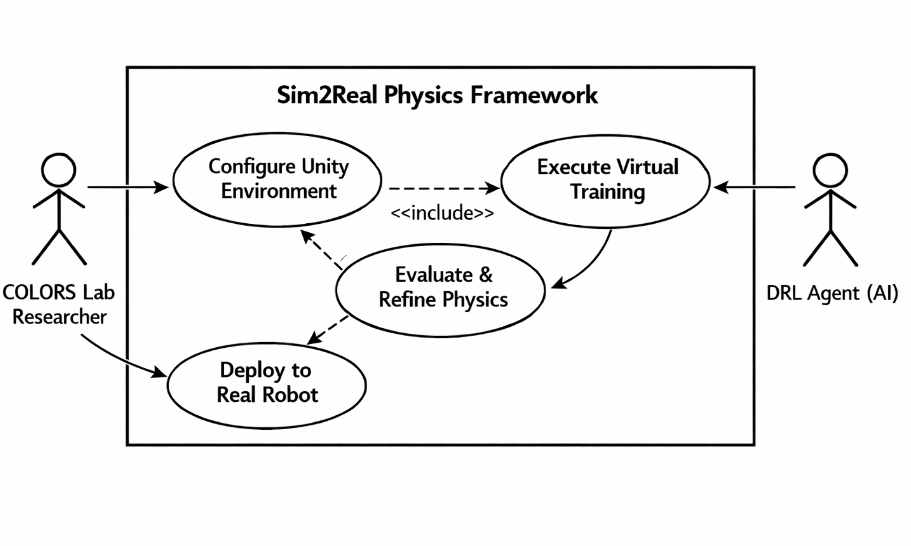
\includegraphics[width=0.8\textwidth]{usecase.png}
\caption{Use Case Diagram illustrating the iterative Sim2Real training pipeline.}
\label{fig:usecase}
\end{figure}
\chapter{DESIGN}

\section{Information Structure}
ER Diagrams.

\section{Information Flow}
Activity diagrams, sequence diagrams, Business Process Modeling Notation.

\section{System Design}
Class diagrams, module diagrams.

\section{User Interface Design (if applicable)}

\chapter{IMPLEMENTATION AND TESTING}
\section{Implementation}
\section{Testing}
\section{Deployment}
Deployment diagram, building instructions, docker/kubernetes, readme, system manual and user manual

\chapter{RESULTS}

\chapter{CONCLUSION}

Citation examples: \cite{conference1}, \cite{article1}, \cite{book1}, \cite{mit}. Footnote example\footnote{More details: {\url{https://www.cmpe.boun.edu.tr/}}}. Referring to figures and tables: Figure \ref{fig:boun}. Table \ref{table:shortTable}.

\begin{figure}[h!]
\centering
\includegraphics[width=0.4\textwidth]{figures/bu-logo.png}
\caption{Figure caption}
\label{fig:boun}
\end{figure}

\begin{table}[thbp]
\vskip\baselineskip 
\caption[Sample table]{Table caption.}
\begin{center}
\begin{tabular}{|c|c|c|} \hline
 & \textbf{Header 1}& \textbf{Header 2}\\\hline
\textbf{Row 1} & 100  & 300 \\\hline
\textbf{Row 2} & 200  & 400 \\\hline
\end{tabular}
\label{table:shortTable}
\end{center}
\end{table}

\bibliographystyle{styles/fbe_tez_v11}
\bibliography{references}

\appendix	
\chapter{SAMPLE APPENDIX}
Contents of the appendix.

\end{document}